\documentclass{beamer}
\usepackage{amsfonts,amsmath,oldgerm}
\usepackage{graphicx}
\usepackage{hyperref}

\usepackage[backend=biber]{biblatex}
\addbibresource{presentation.bib}
\AtBeginBibliography{\small}

\usetheme{sintef}

\newcommand{\testcolor}[1]{\colorbox{#1}{\textcolor{#1}{test}}~\texttt{#1}}

\usefonttheme[onlymath]{serif}

\titlebackground*{assets/background}

\newcommand{\hrefcol}[2]{\textcolor{cyan}{\href{#1}{$#2$}}}


\title{ReConPatch : self-supervision for patch-based anomaly detection}
\subtitle{Computer Vision}
\course{Master's Degree in Artificial Intelligence and Robotics}

\author{\href{mailto:loi.1940849@studenti.uniroma1.it}{Dario Loi} \hspace{1em} \href{mailto:muia.1938610@studenti.uniroma1.it}{Elena Muiá} \hspace{1em} \href{mailto:doku.1938629@studenti.uniroma1.it}{Martina Doku}\\}
\IDnumber{1940849 \hspace{2em} 1938610 \hspace{2em} 1938629}
\date{Academic Year 2023/2024}

\begin{document}
\maketitle

\section{Introduction}
\begin{frame}{Introduction}
      \textbf{Anomaly detection} is a crucial task in many real-world applications,
       such as medical imaging, surveillance, and quality control.\newline 


        In this work, we implement a \textbf{self-supervised} method for anomaly detection
         on industrial images, based on contrastive learning and patch-based
          representations.\newline

          We propose a \textbf{generalized approach} to anomaly detection that can be applied
           to different types of images and anomalies.
          
\end{frame}
\begin{frame}{Objective}
      The goal of this work is to implement a generalized version of the \textbf{Reconpatch} \cite{reconpatch} paper, 
      which defines
       a method for anomaly detection that can be applied to a wide range of industrial images and anomalies.\newline

        We aim to create a \textbf{generalized} model that is 
        trained in a \textbf{self-supervised} manner, on all the normal images of the
         dataset simultaneusly unlike the traditional per-category training.\newline

          The model should be able to detect anomalies in images of unseen categories
           and anomalies, without the need for any labeled data.
\end{frame}
\section{Data}
\begin{frame}{Data}
\begin{columns}
\begin{column}{0.7\textwidth}
      We worked on the \textbf{MVTec AD} \cite{mvtecad} dataset by MVTec Software GmbH (2019), which is a
       widely used benchmark for anomaly detection in industrial images.\newline

        The dataset contains images of \textbf{15 object categories}, each with a
         set of normal and anomalous images.
          The anomalies are introduced by adding various types of defects to the
           normal images, such as scratches, holes, and dents.
\end{column}
           \begin{column}{0.3\textwidth}
            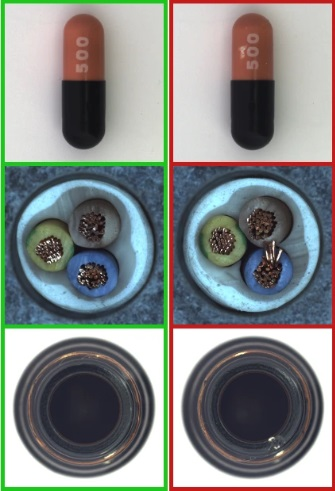
\includegraphics[width=\textwidth]
            {assets/mvtec}
            \end{column}
            \end{columns}
                  
\end{frame}
\begin{frame}{Data}
      Each of the defective images has a corresponding \textbf{ground truth mask},
       which indicates the location of the anomaly in the image.\newline
            \center
       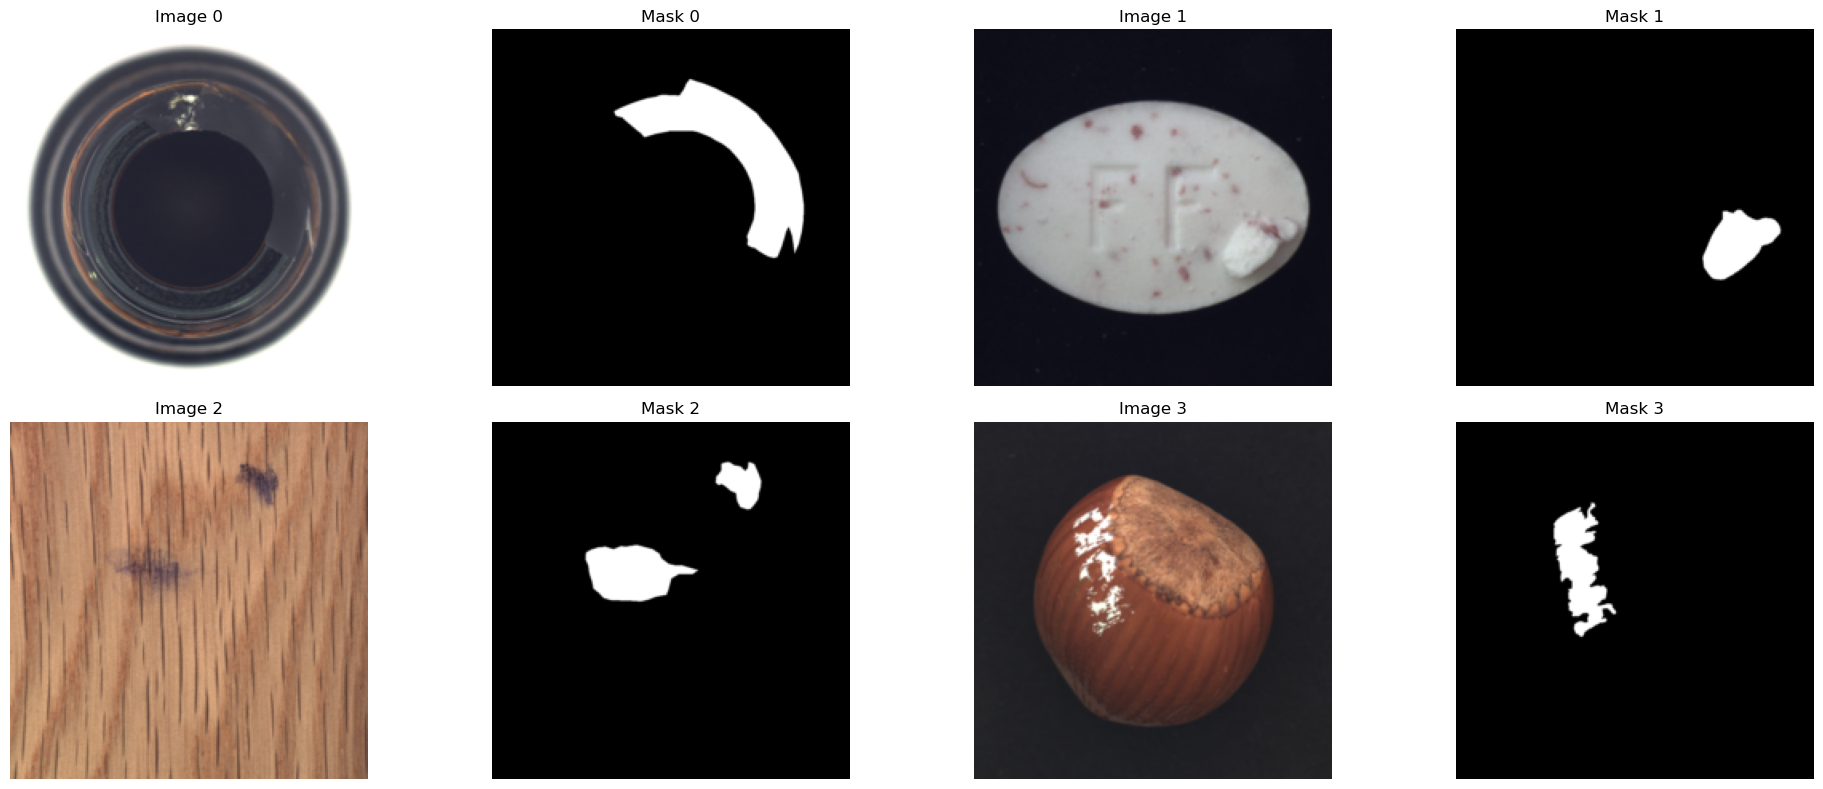
\includegraphics[width=0.9\textwidth]
            {assets/masks}
\end{frame}


\section{Method}
\begin{frame}{Self-Supervised Learning}
      \begin{itemize}
          \item A type of learning where the system learns to predict often through
           pretext tasks that don't require labeled data.
              \item The model is trained on the normal images of the dataset, without
               any information about the anomalies.
                  \item The model learns to encode the normal images in a way that
                   captures the underlying structure of the data.
                      \item During inference, the model can detect anomalies by
                       identifying images that deviate from the learned Embedding.
          \end{itemize}
  \end{frame}
\begin{frame}{Patch-based Anomaly Detection}
      \begin{itemize}
          \item The \textbf{loss $\mathcal{L}$} on which the model is trained is based on the similarity
           between patches of the same image.
           \begin{equation} \mathcal{L} = \frac{1}{N}\sum_{i=1}^{N} \sum_{j=1}^{N} 
            \omega_{ij}\delta_{ij}^2 + (1 - \omega_{ij})\max(0, m - \delta_{ij})^2
      \end{equation}
      where:
      \begin{itemize}
      \item $\delta_{ij}$ denote the relative distance between embedding vectors in a mini-batch
      \item $\omega_{ij}$ indicates the similarity between two patch-level features
      \item $m$ is the margin parameter
\end{itemize}
\end{itemize}
\end{frame}
\begin{frame}{Similarity}
      \begin{itemize}
              \item The \textbf{similarity $\omega$} between two patches is computed using two different
               measures: contextual similarity and pairwise similarity.
              \item The final similarity is computed as a weighted average of the two
               measures:
                  \begin{equation}
                         \omega_{ij} = \alpha\omega_{ij}^{contextual} + (1 - \alpha)\omega_{ij}^{pairwise}
                  \end{equation}
                  where $\alpha$ is a hyperparameter that controls the contribution of
                   each measure.
                  \end{itemize}
  \end{frame}
\begin{frame}{Similarity Measure}
      \begin{itemize}
              \item \textbf{contextual similarity} \begin{equation}
                  \omega_{ij}^{contextual} = \frac{1}{2}(\hat{\omega_{ij}}^{contextual} + \hat{\omega_{ji}}^{contextual})
              \end{equation}
              \begin{equation}
                  \hat{\omega}_{ij}^{contextual} = \begin{cases}
                      \frac{|\mathcal{N}_k(i) \cap \mathcal{N}_k(j)|}{|\mathcal{N}_k(i)|} & \text{if } j \in \mathcal{N}_k(i)\\
                      0 & \text{otherwise}
                  \end{cases}
                  \end{equation}
              \item \textbf{pairwise similarity} \begin{equation}
                  \omega_{ij}^{pairwise} = \exp(-\frac{||\tilde{z}_i - \tilde{z}_j||^2_2}{\sigma})
                  \end{equation}
                  where:
                  \begin{itemize}
                      \item $\tilde{z}_i$ is the embedding of patch $i$ 
                      \item $\sigma$ is a hyperparameter that controls the smoothness of the similarity function.
              \end{itemize}
              \end{itemize}
  \end{frame}
  \begin{frame}{Patch-Level Features Extraction}
        \begin{itemize}
                \item The model uses a pre-trained \textbf{WideResNet-50}\cite{wideresnet} to extract
                 the patch-level features from the input images.
                \item The features are extracted from the \textbf{last convolutional layer} of the network.
                \item The features are then \textbf{flattened} and passed through a double \textbf{representation learning network}
                 to train the feature embeddings.
                \end{itemize}
  \end{frame}
  \begin{frame}{Double network structure}
      \begin{itemize}
              \item The model consists of  an online network and a target network.
              \item \textbf{Online network}:
                  \begin{itemize}
                          \item  The online network itakes as input the patch-level features.
                          \item The online netwrok processes the features through a representation and projection
                           layers and sends the result as input of the loss function.
                          \item The online network is updated during training using the contrastive loss.
                          
                          
                          \end{itemize}
                  \item \textbf{Target network}:
                          \begin{itemize}
                                \item The target network is a copy of the online network that is used to compute the similarity between patches.
                                \item The target network sends the result of the similarity computation as input of the loss function.
                                \item The target network is updated using an exponential moving average of the online network's parameters.
                                \end{itemize}

                  \end{itemize}
      \end{frame}
\section{Experiments}
\begin{frame}{Model}
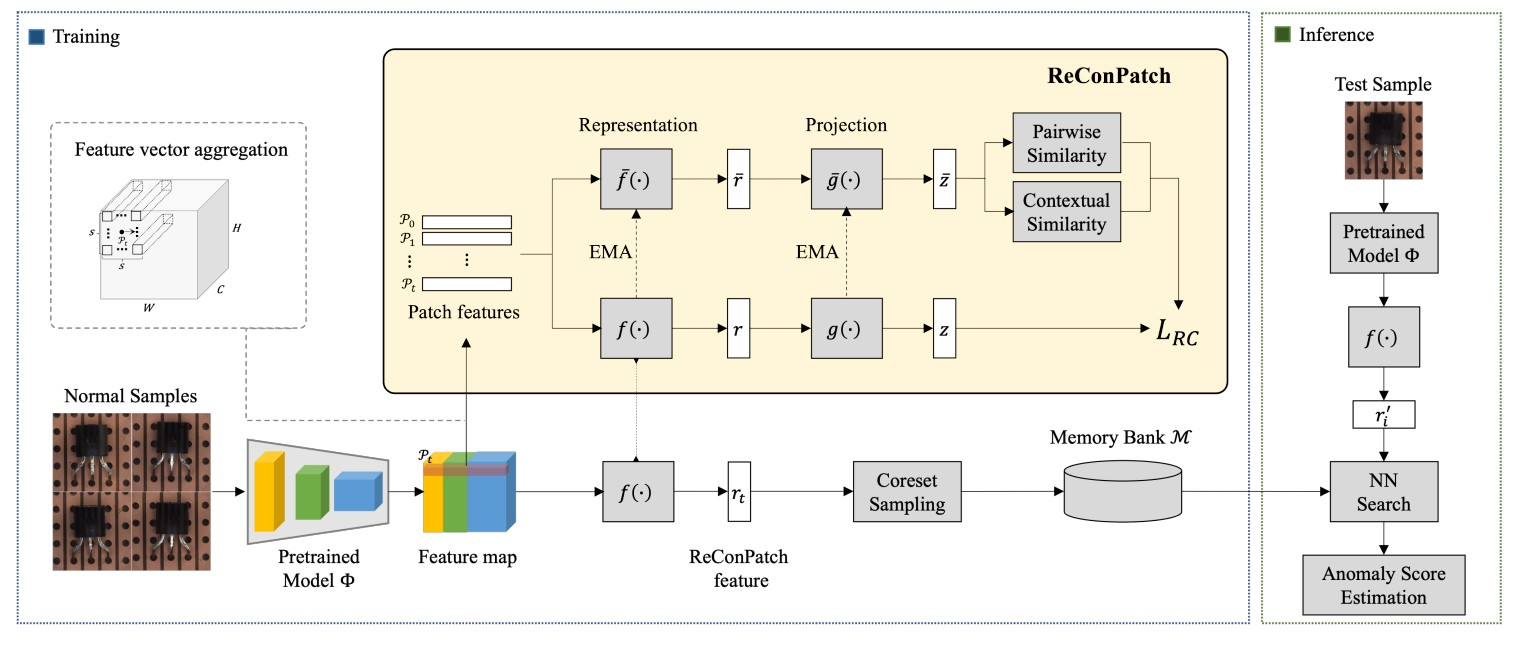
\includegraphics[width=\textwidth]
{assets/model}
\end{frame}
\begin{frame}{Training}
      \begin{itemize}
              \item The model is trained on the normal images of the dataset 
              using the contrastive loss.
              \item The \textbf{optimizer} used is Adam with a learning rate of $10^{-4}$.
              \item The \textbf{batch size} is set to 32
              \item The model is trained for a total of \textbf{100 epochs}, with an \textbf{early stopping
               criterion} based on the validation loss, with a patience of 10 epochs.
              \end{itemize}
\end{frame}

\begin{frame}{Inference Pipeline}
      \begin{itemize}
              \item During inference, the model is used to encode the test images
               and compute the anomaly score for each patch \cite{patchcore}.
              \item  After training a \textbf{coreset} of features $r^*$ is selected
              using a greedy approximation algorith and stored in 
              a \textbf{Memory Bank} $\mathcal{M}$.
                  \item The \textbf{anomaly score} for each patch is computed as:
                  \begin{equation}
                      s_i = (1- \frac{e^{s'_i}}{\sum_{r' \in \mathcal{N}_{b(r^*)}}e^{\mathcal{D}(z_i, r')}}) \cdot \mathcal{D}(z_i, r^*)
                  \end{equation}
                  where:
                  \begin{itemize}
                      \item $s'_i$ is the similarity between the patch and its nearest neighbor in the Memory Bank
                      \item $\mathcal{N}_{b(r^*)}$ is the set of neighbors of $r^*$ in the Memory Bank
                      \item $\mathcal{D}$ is the distance function
                      \end{itemize}
              \end{itemize}
\end{frame}
\begin{frame}{Metrics}
      \begin{itemize}
              \item The performance of the model is evaluated using the \textbf{Area Under the
               Receiver Operating Characteristic curve (AUC-ROC)} 
               \begin{equation}
                   \text{AUC-ROC} =  \int_{0}^{1} \text{TPR}(FPR)  d(\text{FPR})
                  \end{equation}
                  where:
                  \begin{itemize}
                      \item $TPR$ is the True Positive Rate
                      \item $FPR$ is the False Positive Rate
                      \end{itemize}
                  
                  \item The AUC-ROC was measured both on the \textbf{patch-level} and 
                  the \textbf{image-level}.
              \end{itemize}
\end{frame}
\begin{frame}{Results}
      We evaluated the model on the \textbf{MVTec AD}\cite{mvtecad} dataset using the \textbf{AUROC} metric.
      We obtained an \textbf{AUROC} of \textbf{0.60} on the \textbf{patch-level} and \textbf{0.70} 
      on the \textbf{image-level}.
\end{frame}
\begin{frame}{Embedding}
\end{frame}
\section{Conclusion}

\begin{frame}{Conclusion}
      We have presented a self-supervised method for anomaly detection based
 on patch-based representations. The model is trained on the normal images
  of the dataset, and is able to detect 
  anomalies in images of all categories and anomalies, obtaining an increased 
  generality compared to traditional methods.
\end{frame}
\begin{frame}{Future Work}
      There are still several aspects of the model that can be improved, to 
      increase the performance and generality of the model:
      \begin{itemize}
              \item \textbf{Hyperparameter tuning}: The model has several hyperparameters
               that can be tuned to improve performance.
              \item \textbf{Heavier training}: The model can be trained for longer
               or with a larger batch size to improve performance.
               \item \textbf{Anomaly scores}: The anomaly scores can be further refined
                to improve the detection of anomalies.
                \end{itemize}
\end{frame}

\begin{frame}[allowframebreaks, noframenumbering]{References}
\printbibliography
\end{frame}


\backmatter
\end{document}